\documentclass{article}
%%%%%%%%%%%%%%%%%%%%%%%%%%%%%%%%%%%%%%%%%%%%%%%%%%%%%%%%%%%%%%%%%%%%%%%%%%%%%%%%%%%%%%%%%%%%%%%%%%%%%%%%%
\usepackage{csquotes,xpatch}% recommended
\usepackage[backend=bibtex,
style=authoryear-comp,
sortcites=false,
maxbibnames=5,maxcitenames=2,
firstinits=true,
natbib=true,
]{biblatex}

\addbibresource{refs.bib}

% natbib = true: add comma between author and year
% firstinits: for first name initials in bibliography
\renewcommand{\postnotedelim}{ } % remove comma in post citation in autocite
%\addbibresource{refs.bib}
%%%%%%%%%%%%%%%%%%%%%%%%%%%%%%%%%%%%%%%%%%%%%%%%%%%%%%%%%%%%%%%%%%%%%%%%%%%%%%%%%%%%%%%%%%%%%%%%%%%%%%%%%

% Combine label and labelyear links
\xpatchbibmacro{cite}
{\usebibmacro{cite:label}%
	\setunit{\addspace}%
	\usebibmacro{cite:labelyear+extrayear}}
{\printtext[bibhyperref]{%
		\DeclareFieldAlias{bibhyperref}{default}%
		\usebibmacro{cite:label}%
		\setunit{\addspace}%
		\usebibmacro{cite:labelyear+extrayear}}}{}{}

% Include labelname in labelyear link
\xpatchbibmacro{cite}
{\printnames{labelname}%
	\setunit{\nameyeardelim}%
	\usebibmacro{cite:labelyear+extrayear}}
{\printtext[bibhyperref]{%
		\DeclareFieldAlias{bibhyperref}{default}%
		\printnames{labelname}%
		\setunit{\nameyeardelim}%
		\usebibmacro{cite:labelyear+extrayear}}}{}{}

% Access hyperref's citation link start/end commands
\makeatletter
\protected\def\blx@imc@biblinkstart{%
	\@ifnextchar[%]
	{\blx@biblinkstart}
	{\blx@biblinkstart[\abx@field@entrykey]}}
\def\blx@biblinkstart[#1]{%
	\blx@sfsave\hyper@natlinkstart{\the\c@refsection @#1}\blx@sfrest}
\protected\def\blx@imc@biblinkend{%
	\blx@sfsave\hyper@natlinkend\blx@sfrest}
\blx@regimcs{\biblinkstart \biblinkend}
\makeatother

\newbool{cbx:link}

% Include parentheses around labelyear in \textcite only in
% single citations without pre- and postnotes
\def\iflinkparens{%
	\ifboolexpr{ test {\ifnumequal{\value{multicitetotal}}{0}} and
		test {\ifnumequal{\value{citetotal}}{1}} and
		test {\iffieldundef{prenote}} and
		test {\iffieldundef{postnote}} }}

\xpatchbibmacro{textcite}
{\printnames{labelname}}
{\iflinkparens
	{\DeclareFieldAlias{bibhyperref}{default}%
		\global\booltrue{cbx:link}\biblinkstart%
		\printnames{labelname}}
	{\printtext[bibhyperref]{\printnames{labelname}}}}{}{}

\xpatchbibmacro{textcite}
{\usebibmacro{cite:label}}
{\iflinkparens
	{\DeclareFieldAlias{bibhyperref}{default}%
		\global\booltrue{cbx:link}\biblinkstart%
		\usebibmacro{cite:label}}
	{\usebibmacro{cite:label}}}{}{}

\xpretobibmacro{textcite:postnote}
{\ifbool{cbx:link}% patch 2.7+
	{\ifbool{cbx:parens}
		{\bibcloseparen\global\boolfalse{cbx:parens}}
		{}%
		\biblinkend\global\boolfalse{cbx:link}}
	{}}
{}
{\xpatchbibmacro{textcite}% patch earlier releases
	{\setunit{%
			\ifbool{cbx:parens}
			{\bibcloseparen\global\boolfalse{cbx:parens}}
			{}%
			\multicitedelim}}
	{\ifbool{cbx:link}
		{\ifbool{cbx:parens}
			{\bibcloseparen\global\boolfalse{cbx:parens}}
			{}%
			\biblinkend\global\boolfalse{cbx:link}}
		{}%
		\setunit{%
			\ifbool{cbx:parens}
			{\bibcloseparen\global\boolfalse{cbx:parens}}
			{}%
			\multicitedelim}}
	{}{}}
%%%%%%%%%%%%%%%%%%%%%%%%%%%%%%%%%%%%%%%%%%%%%%%%%%%%%%%%%%%%%%%%%%%%%%%%%%%%%%%%%%%%%%%%%%%%%%%%%%%%%%%%%
\DeclareNameAlias{sortname}{last-first} % last name first
\renewbibmacro{in:}{} % remove in: before journal

%%%%%%%%%%%%%%%%%%%%%%%%%%%%%%%%%%%%%%%%%%%%%%%%%%%%%%%%%%%%%%%%%%%%%%%%%%%%%%%%%%%%%%%%%%%%%%%%%%%%%%%%%
\usepackage{graphicx}
\usepackage{epstopdf} 
%%%%%%%%%%%%%%%%%%%%%%%%%%%%%%%%%%%%%%%%%%%%%%%%%%%%%%%%%%%%%%%%%%%%%%%%%%%%%%%%%%%%%%%%%%%%%%%%%%%%%%%%%
\usepackage{calrsfs}
\usepackage{physics}
\usepackage{mathtools}  
\usepackage{amsmath}
\usepackage{amssymb}
\usepackage{tabulary}
\usepackage{booktabs}
\usepackage{hyperref}
%%%%%%%%%%%%%%%%%%%%%%%%%%%%%%%%%%%%%%%%%%%%%%%%%%%%%%%%%%%%%%%%%%%%%%%%%%%%%%%%%%%%%%%%%%%%%%%%%%%%%%%%%
%\usepackage{chngcntr}
%\numberwithin{equation}{chapter}
%\counterwithin{figure}{chapter}
%%%%%%%%%%%%%%%%%%%%%%%%%%%%%%%%%%%%%%%%%%%%%%%%%%%%%%%%%%%%%%%%%%%%%%%%%%%%%%%%%%%%%%%%%%%%%%%%%%%%%%%%%
\setlength{\parindent}{2em}
\setlength{\parskip}{1em}

\linespread{1.6}
\usepackage{geometry}
\geometry{
	a4paper,
	total={134mm,225mm},
	left=38mm,
	top=35mm,
	headsep=.5in
}
\raggedbottom
%%%%%%%%%%%%%%%%%%%%%%%%%%%%%%%%%%%%%%%%%%%%%%%%%%%%%%%%%%%%%%%%%%%%%%%%%%%%%%%%%%%%%%%%%%%%%%%%%%%%%%%%%
\usepackage{blindtext}
\usepackage{ragged2e}
\usepackage{float}

\usepackage{epstopdf}
\usepackage{empheq} 

\usepackage{array}
\hypersetup{
	colorlinks
}
%%%%%%%%%%%%%%%%%%%%%%%%%%%%%%%%%%%%%%%%%%%%%%%%%%%%%%%%%%%%%%%%%%%%%%%%%%%%%%%%%%%%%%%%%%%%%%%%%%%%%%%%%
\usepackage{graphics}
\graphicspath{ {figures/} }
\renewcommand{\listfigurename}{List of figures}

\usepackage[labelfont=bf,justification=justified,singlelinecheck=false]{caption}
\captionsetup[figure]{name=Fig. ,labelsep=period}
\captionsetup[table]{labelsep=period}
\captionsetup[figure]{labelfont={bf},labelformat={default},labelsep=period,name={Fig.}}
%%%%%%%%%%%%%%%%%%%%%%%%%%%%%%%%%%%%%%%%%%%%%%%%%%%%%%%%%%%%%%%%%%%%%%%%%%%%%%%%%%%%%%%%%%%%%%%%%%%%%%%%%
\usepackage{array}
\usepackage{longtable}
\usepackage{xcolor}

\usepackage{comment}

\usepackage{enumitem}

\usepackage{wrapfig}
%%%%%%%%%%%%%%%%%%%%%%%%%%%%%%%%%%%%%%%%%%%%%%%%%%%%%%%%%%%%%%%%%%%%%%%%%%%%%%%%%%%%%%%%%%%%%%%%%%%%%%%%%
\usepackage{titlesec}

\titlespacing*{\section}
{0pt}{1ex plus .5ex minus .2ex}{.5ex plus .2ex}
\titlespacing*{\subsection}
{0pt}{0.5ex plus .5ex minus .2ex}{.5ex plus .2ex}
%\titlespacing*{\subparagraph}
%{0pt}{2.5ex plus 1ex minus .2ex}{1.3ex plus .2ex}

\setcounter{secnumdepth}{4}
\setcounter{tocdepth}{4}

\newcommand{\hsp}{\hspace{5pt}}

\titleformat{\section}[block]{\bfseries\large}{\thesection}{1em}{}
\titleformat{\subsection}[block]{\bfseries\itshape}{\thesubsection}{1em}{}


%\titleformat{\subsubsection}
%{\normalfont\normalsize\itshape}{\thesubsubsection}{1em}{}
%\titleformat{\subparagraph}[runin]
%{\itshape\normalsize}{\thesubparagraph}{1em}{}

%%%%%%%%%%%%%%%%%%%%%%%%%%%%%%%%%%%%%%%%%%%%%%%%%%%%%%%%%%%%%%%%%%%%%%%%%%%%%%%%%%%%%%%%%%%%%%%%%%%%%%%%%
\usepackage{subcaption}
\usepackage{bbm}
\usepackage{tabularx}
%%%%%%%%%%%%%%%%%%%%%%%%%%%%%%%%%%%%%%%%%%%%%%%%%%%%%%%%%%%%%%%%%%%%%%%%%%%%%%%%%%%%%%%%%%%%%%%%%%%%%%%%%
\definecolor{mycolor}{RGB}{207,42,40}
\AtBeginDocument{\hypersetup{citecolor=violet, linkcolor = mycolor}}

\usepackage{indentfirst}


%%%%%%%%%%%%%%%%%%%%%%%%%%%%%%%%%%%%%%%%%%%%%%%%%%%%%%%%%%%%%%%%%%%%%%%%%%%%%%%%%%%%%%%%%%%%%%%%%%%%%%%%
\setlength{\belowcaptionskip}{-20pt}
\begin{document}
	
	\sloppy
	
%%%%%%%%%%%%%%%%%%%%%%%%%%%%%%%%%%%%%%%%%%%%%%%%%%%%%%%%%%%%%%%%%%%%%%%%%%%%%%%%%%%%%%%%%%%%%%%%%%%%%%%%%
	\begin{center}	
		\Large
		\textbf{Review of \textcite{aghasi2020fast}: \\
			Fast Convex Pruning of Deep Neural Networks}\\
		\large
		Apostolos Psaros\\	
%		\today
%		July 10, 2020
	\end{center}
	\vskip 0.5in
	
%%%%%%%%%%%%%%%%%%%%%%%%%%%%%%%%%%%%%%%%%%%%%%%%%%%%%%%%%%%%%%%%%%%%%%%%%%%%%%%%%%%%%%%%%%%%%%%%%%%%%%%%%

\section{Motivation}
\begin{itemize}
	\item Increasing size/flexibility of NNs leads to increasing complexity and in turn to overfitting 
	\item Regularization is used to reduce overfitting. Typical approaches include:
	\begin{enumerate}
		\item hard/soft constraints on the parameters (e.g., weight decay)
		\item ensembling
		\item data augmentation
		\item pruning
	\end{enumerate}
	\item \textcite{goodfellow2016deep}: ``We almost always find that the best fitting model (in the sense of generalization error) is a large model that has been regularized appropriately''
	\item An additional problem of increasing the size of NNs is the related increase in storage requirements and the number of floating point operations (FLOPs)
	\item It becomes hard to apply the models on mobile platforms with limited memory and processing units
\end{itemize}

\section{Pruning background}
\begin{itemize}
	\item Motivation: Significantly redundant parametrizations: sparser weight matrices may result in similar or better performance
	\item Commonly (e.g., \cite{han2015learning}), pruning consists of 3 stages:
	\begin{enumerate}
		\item standard training (we learn what neuron connections are important)
		\item deleting of unimportant connections (magnitude below some threshold): set corresponding weights to zero
		\item retraining the network with the remaining connections (often called fine-tuning)
	\end{enumerate}
	\item Net-Trim stages: 
	\begin{enumerate}
		\item standard training
		\item for each layer replacing weight matrix by a sparser one that produces approximately the same layer outputs (internal features)
		\item fine-tuning (optional)
	\end{enumerate}
\end{itemize}

\section{Introduction to Net-Trim}

\begin{itemize}
	\item Consider an FFN with $L$ layers
	\begin{figure}[H]
		\centering
		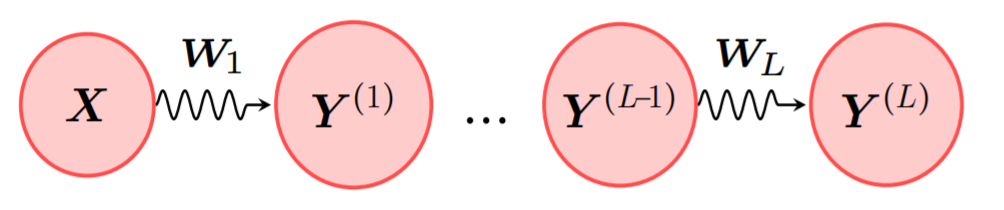
\includegraphics[width=0.6\linewidth]{./figs/FFN_1.png}  
		\caption{Fig 2 from \textcite{aghasi2017nettrim}. In \textcite{aghasi2020fast} X is used in the layers instead of Y.}
		%\label{fig:lr_sched}
	\end{figure}
	\item Each weight matrix $W_l$ is of size $N_{l-1}\times N_l$
	\item layer outputs are given as $X^{(l)} = ReLU(W_l^TX^{(l-1)})$
	\begin{figure}[H]
		\centering
		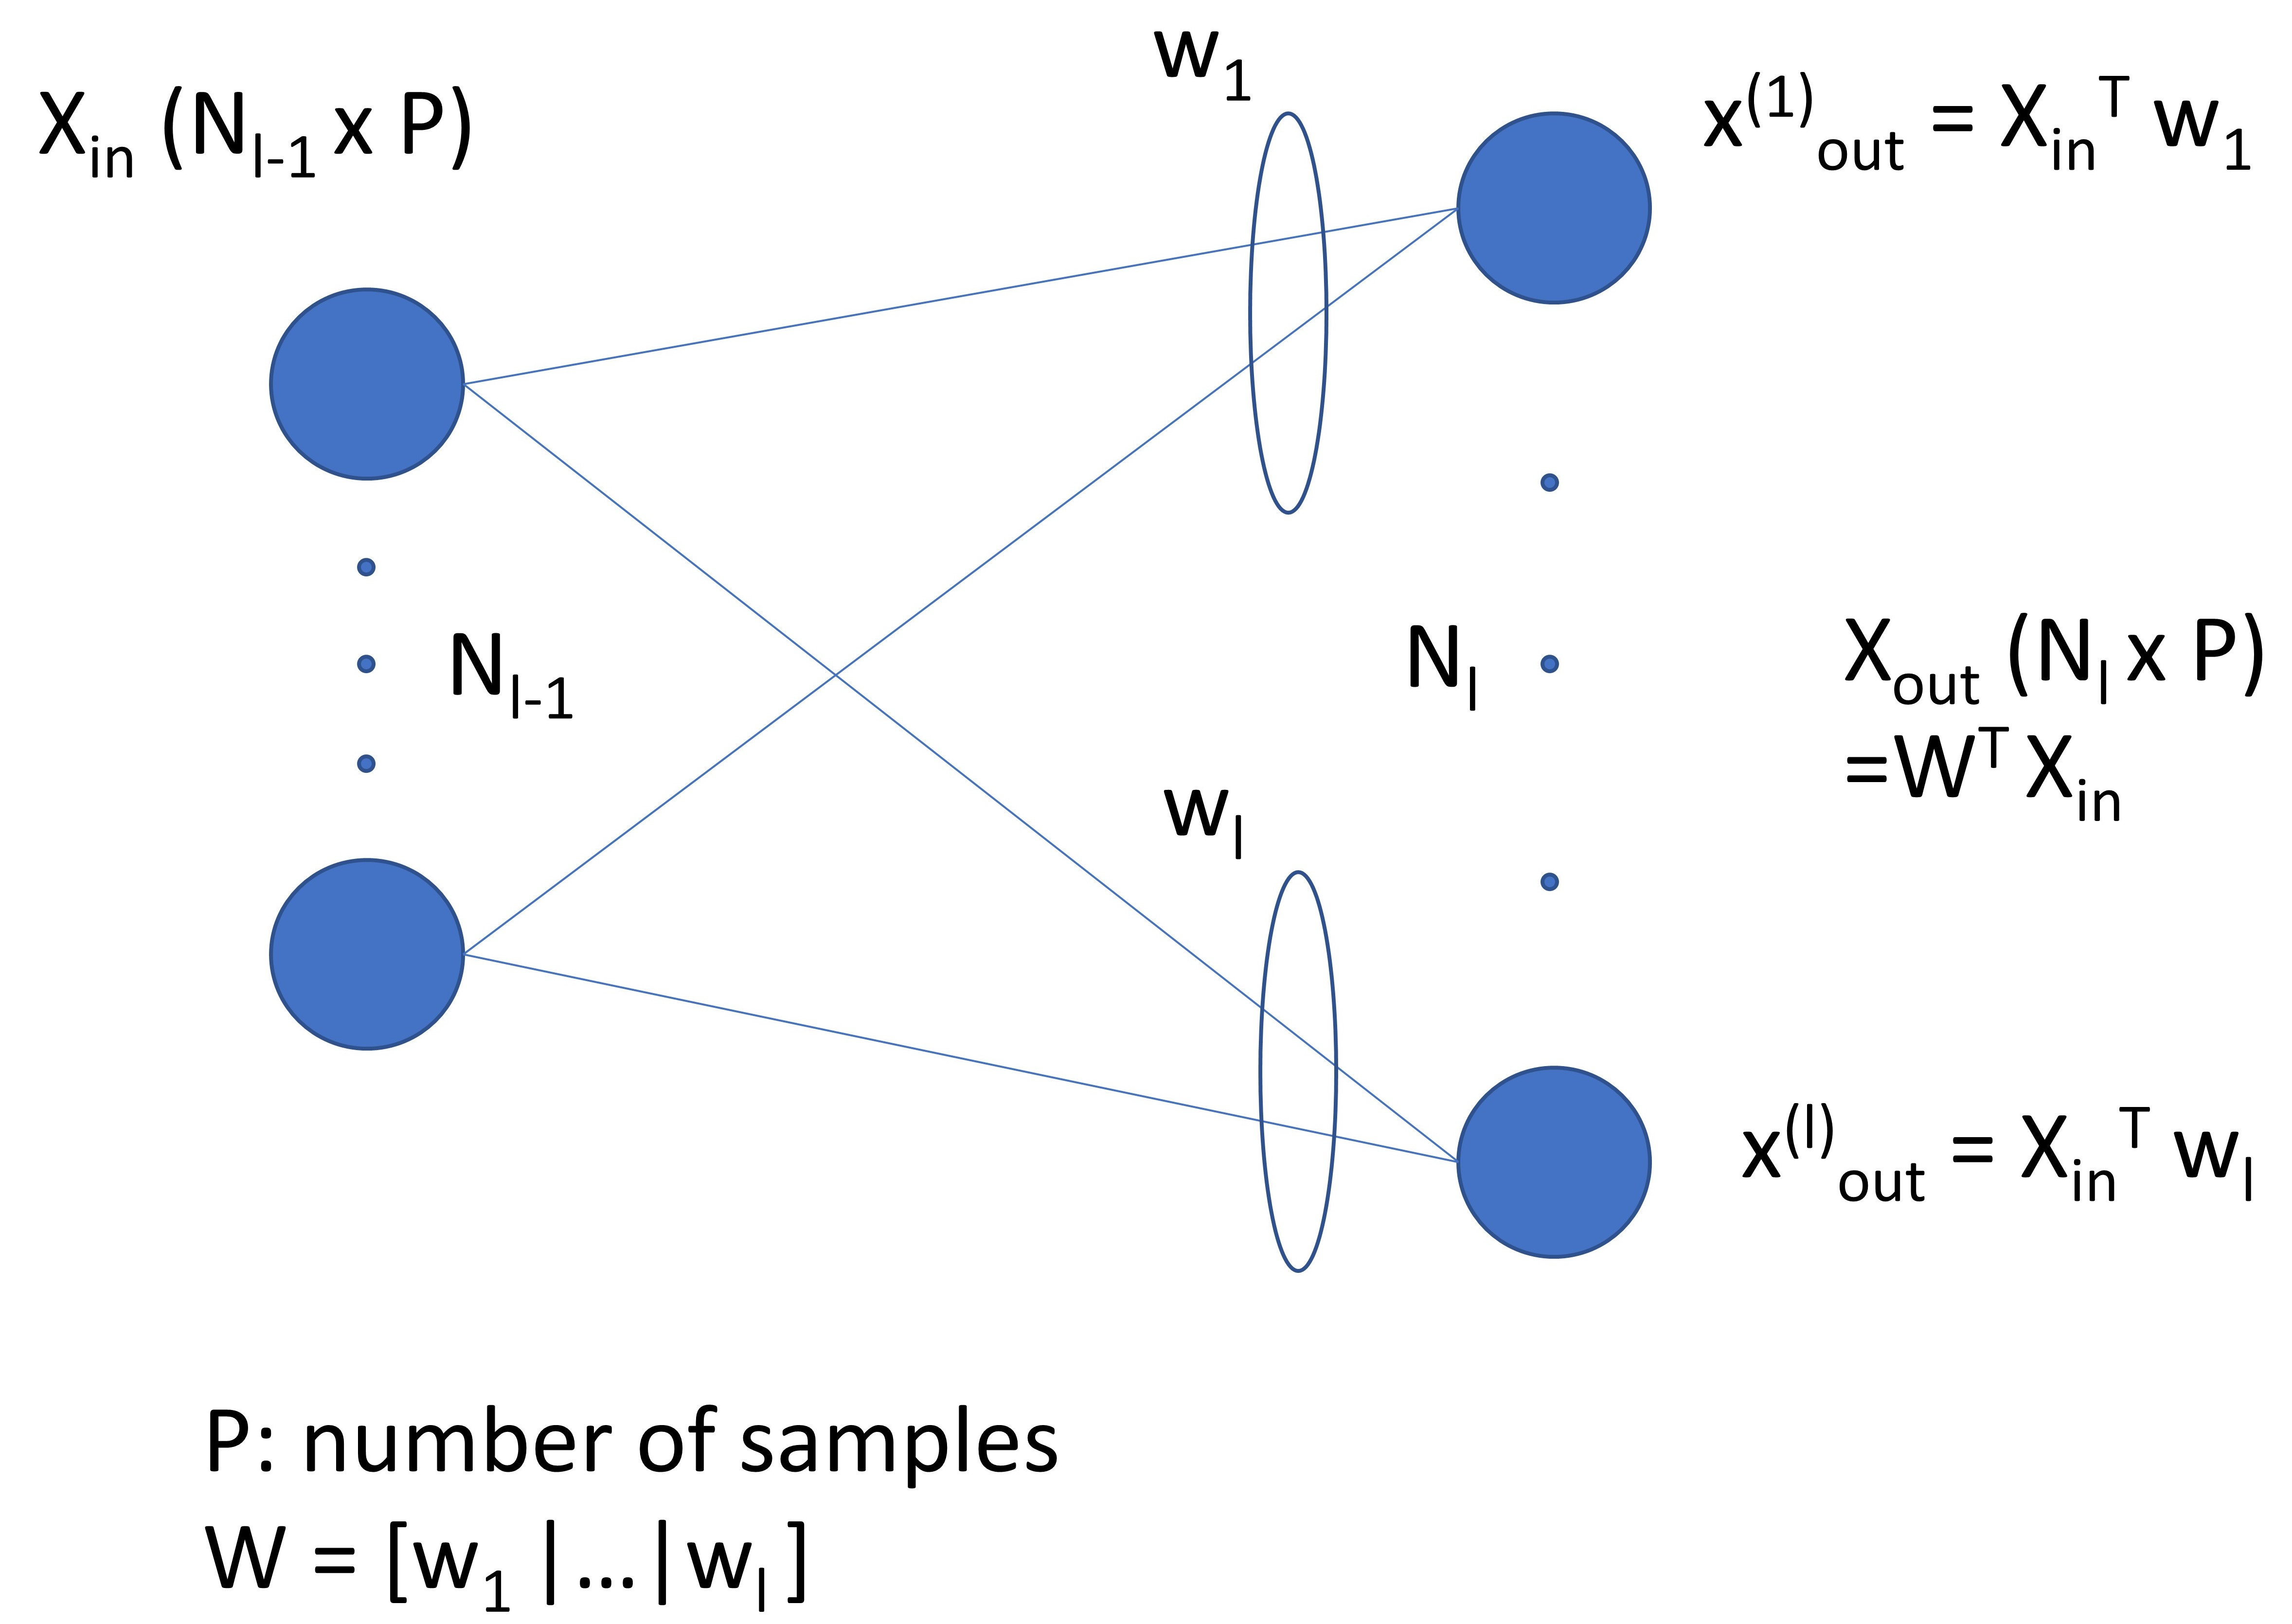
\includegraphics[width=.7\linewidth]{./figs/FFN_2.jpg}  
		\caption{Layer outputs without activation function for simplicity.}
		%\label{fig:lr_sched}
	\end{figure}
	\item For each layer search for a sparser weight matrix:\\ $\min_{}\norm{W}_1 \quad \text{subject to} \quad \norm{ReLU(W^T X_{in}-X_{out})}_F \leq \epsilon $
	\item Similar output (controllable discrepancy $\epsilon$) with smaller $\norm{W}_1$
	\item Convexify constraint: replace $X^{(l)} = ReLU(W_l^TX^{(l-1)})$ by \\
	\begin{equation*}
	\begin{aligned}
		\norm{(W^T X_{in}-X_{out})_{\Omega}}_F & \leq \epsilon \\
		(W^T X_{in})_{\Omega^c} & \leq 0
	\end{aligned}
	\end{equation*}
\setlength{\belowcaptionskip}{-40pt}
	\begin{figure}[H]
	\centering
	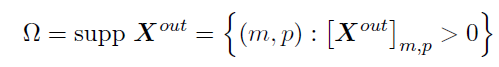
\includegraphics[width=.5\linewidth]{./figs/omega.png}  
	\caption*{}
	%\label{fig:lr_sched}
	\end{figure}
	\begin{itemize}
		\item if an element of $X_{out}$ is greater than zero then it will be unaffected by ReLU. Thus, we require that $W^T X_{in}$ is close to $X_{out}$. This both gives the same result and also avoids ReLU
		\item if an element of $X_{out}$ is less than zero then it will be zeroed out by ReLU. Thus, we require that $W^T X_{in}$ is also less than zero which both gives the same result and also avoids ReLU
	\end{itemize}	
	\item Two frameworks: Parallel and Cascade 
	\begin{enumerate}
		\item Parallel: Each layer is retrained independently based on the inputs-outputs from the original training 
		\begin{itemize}
			\item We can prove that the output discrepancy for each layer is bounded
			
				\begin{figure}[H]
				\centering
				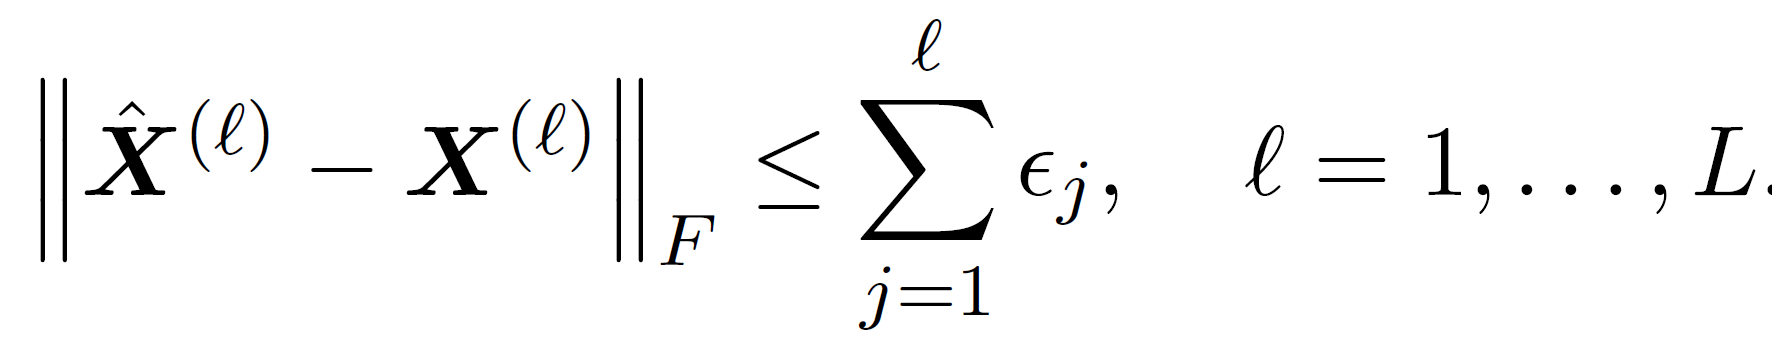
\includegraphics[width=.5\linewidth]{./figs/par_cons.png}  
				\caption*{}
				%\label{fig:lr_sched}
			\end{figure}	
		\setlength{\belowcaptionskip}{-20pt}
			\item Recall that after retraining $\hat{X}$ (not $X$) will be fed to the next layer so we do need the above bound
			\item Retraining of layers can be done in parallel
		\end{itemize}
		\item Cascade: Incorporates the outcome of the previously pruned layers to retrain the next layers
		\begin{itemize}
			\item Similar bound can be proved
			\item Sparser networks at the expense of increased computational cost
		\end{itemize}
	\end{enumerate}
\end{itemize}

\section{Connections with sparse representations/compressed sensing}
\begin{itemize}
	\item Consider an unknown vector $w_{n\times 1}$
	\item We observe linear measurements $y_{m\times 1} = X_{m\times n}w_{n\times 1}+\epsilon$
	\item How can we approximate $w$?
	\item X is usually called sampling matrix
	\begin{itemize}
		\item Often the columns of X correspond to basis vectors sampled at random locations (rows)
		\item In the over-determined case ($m>n$) we use the LSE given as $\hat{w} = (X^TX)^{-1}X^Ty$
		\item Gives the exact solution if there exists one or an approximation if no exact solution exists
		\item In the under-determined case ($m<n$) $X$ does not have full column rank and thus $X^TX$ does not exist. This is the compressed sensing problem
		\item How can we obtain a unique solution? 
		\item If $w$ is sparse enough then we can obtain it by solving $\min_{}\norm{w}_1 \quad \text{subject to} \quad \norm{Xw - y}_2 \leq \epsilon $
		\item We are interested in the true $w$ and sparsity is used as a means for getting it	
		\item Many theoretical results in the 2000s	
	\end{itemize}
	\item Back to Net-Trim: Let's isolate an output neuron of a NN layer
	\begin{figure}[H]
	\centering
	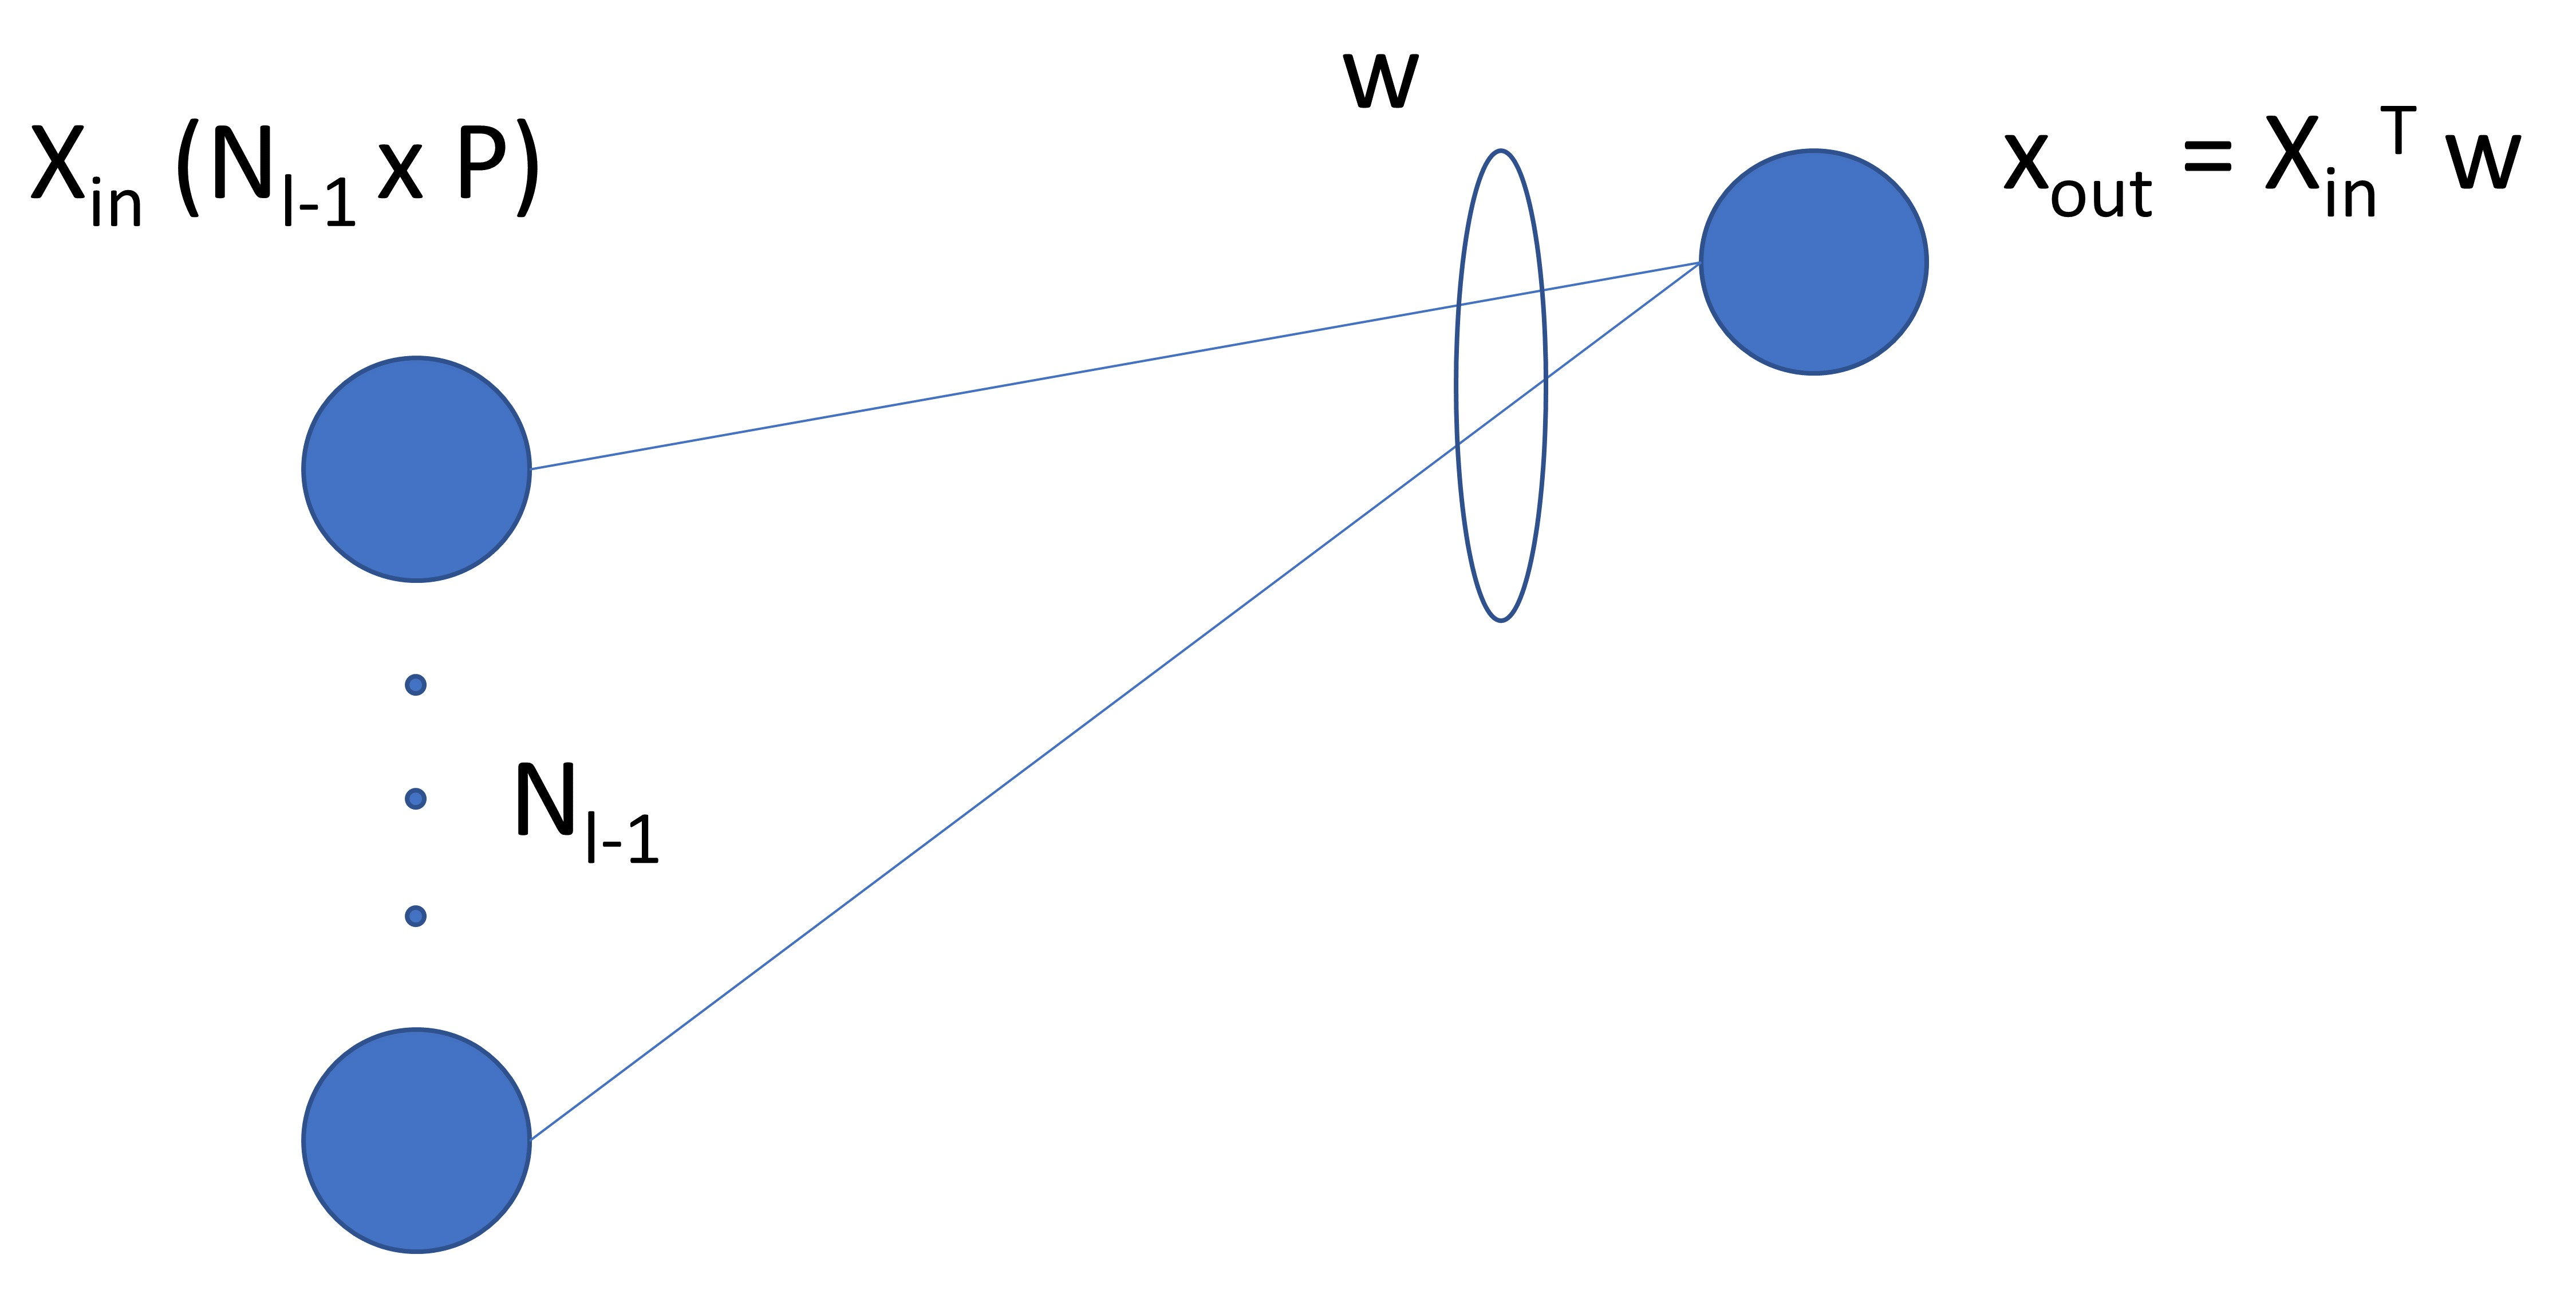
\includegraphics[width=.7\linewidth]{./figs/FFN_3.jpg}  
	\caption*{}
	%\label{fig:lr_sched}
	\end{figure}	
	\item The equation $x_{out} = X_{in}^Tw$ is of the form of $y = Xw$
	\item The sampling matrix is $X_{in}^T$: its columns correspond to different input neurons and its rows to different samples
	\item Can be over/under-determined system
	\item In order to sparsify $w$ we need to \textbf{solve the same minimization problem} as the one solved in compressed sensing
	\item Sparsifying $w$ means reducing the number of connections from the input neurons to a given output neuron
	\item We first reduced the original convex problem with non-convex constraints to a convex one with convex constraints (got rid of ReLU) and then to a series of convex problems (one for each output neuron)
	\item Easier to do theory: we can use the rich compressed sensing theory 
\end{itemize}

\section{Brief review of compressed sensing (underdetermined case)}
\begin{itemize}
	\item Underdetermined system: $y_{m\times 1} = X_{m\times n}w_{n\times 1}$
	\item If $w$ is $s$-sparse then we can obtain it exactly by solving \\
	$ \min \norm{w}_0 \quad \text{subject to} \quad Xw = y $
	\item How do we know that the solution is unique and exact?
	\item $w$ needs to be structured (e.g., sparsity $s = \norm{w}_0 << n$)
	\item $X$ needs to be ``nice'' (e.g., small coherence)
	\item Thus, most related theorems follow these lines: Suppose that $w$ is an unknown $s$-sparse vector and we have observations $y_{m\times 1} = X_{m\times n}w_{n\times 1}$.
	If $s$ is smaller than a number that has to do with some property of $X$, then by solving the $\ell_0$ minimization problem you can get the exact $w$
	\item For example, if $s \leq krank(X)/2$ then the $\ell_0$ minimization problem results in the exact solution $w$ (krank($X$) is the largest number $r$ such that any subset of $r$ columns of $X$ is linearly independent)
	\item Because $X$ is a sampling matrix and corresponds to random observations, these theorems often have a randomness component. For example, if $X$ is a matrix filled with Gaussian i.i.d. samples then $krank(X) = m$ almost surely 	
	\item Thus, most related theorems take this form: Suppose that $w$ is an unknown $s$-sparse vector and we have observations $y_{m\times 1} = X_{m\times n}w_{n\times 1}$ where $X$ is a matrix filled with Gaussian i.i.d. samples. 
	If the number of observations $m$ is larger than a number that is a function of the sparsity $s$, then by solving the $\ell_0$ minimization problem you can get the exact $w$ with high probability
	\item Since solving the $\ell_0$ minimization problem is NP-hard we instead solve the convex alternative which is the $\ell_1$ minimization problem. We can prove similar theorems for this problem
	\item The main theorem of the paper has exactly this form but is more general because it considers also the overdetermined case. 
	Thus without even looking at the proof we can still understand the basic ingredients of the theorem	
\end{itemize} 

\newpage
\section{Main theorem of the paper}
	\begin{figure}[H]
	\centering
	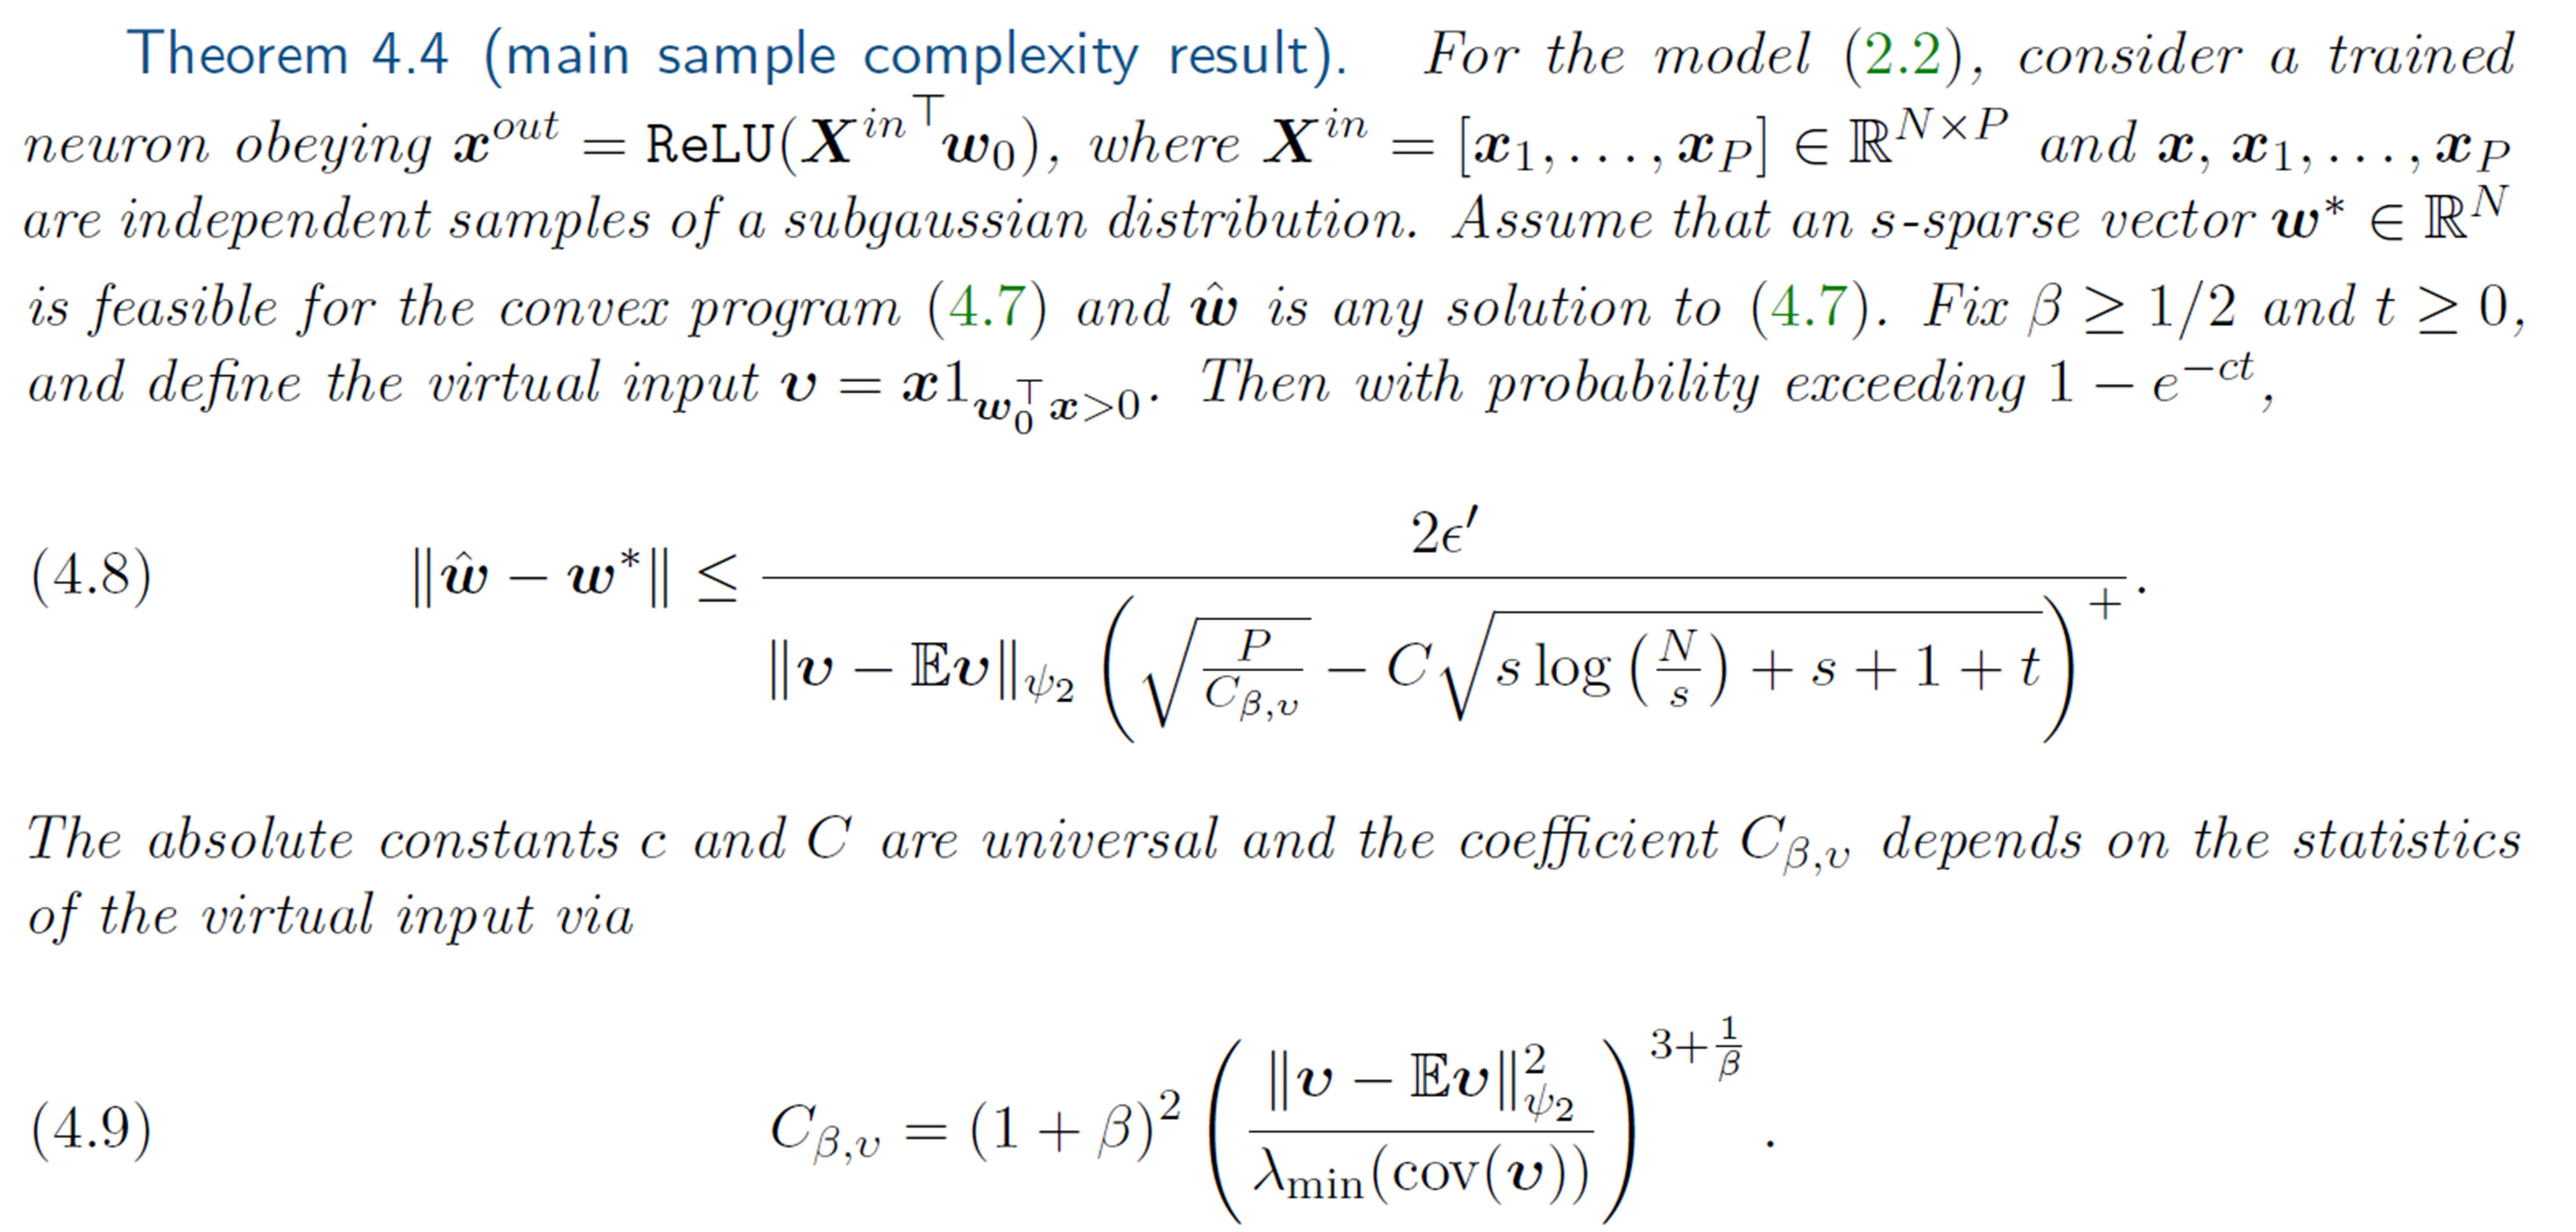
\includegraphics[width=1\linewidth]{./figs/theorem.jpg}  
	\caption*{}
	%\label{fig:lr_sched}
\end{figure}
\setlength{\belowcaptionskip}{-40pt}
	\begin{figure}[H]
	\centering
	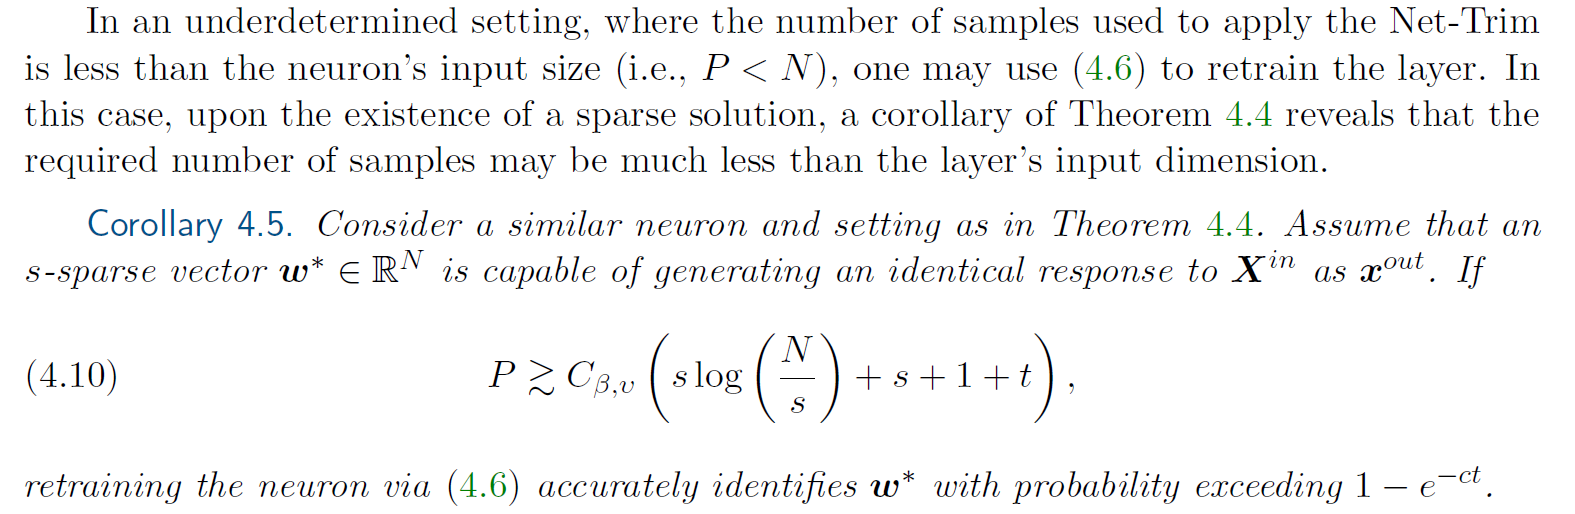
\includegraphics[width=1\linewidth]{./figs/corollary.png}  
	\caption*{}
	%\label{fig:lr_sched}
\end{figure}
\setlength{\belowcaptionskip}{-20pt}

\begin{itemize}
	\item What to remember: If the weight matrix of a layer is indeed redundant and there exists a sparser matrix producing the same outputs, then you can solve the $\ell_1$ minimization problem and approximately obtain this sparser matrix. This is true even if the number of samples you use is less than the number of output neuron connections  
	\item The original minimization problem \textbf{for each layer} is \\
	$\min_{}\norm{W}_1 \quad \text{subject to} \quad \norm{(W^T X_{in}-X_{out})_{\Omega}}_F \leq \epsilon \quad \text{and}\quad (W^T X_{in})_{\Omega^c} \leq 0 $ \\
	but in the theoretical part the problem is divided into a number of smaller minimization problems so that it is easier to provide a theorem. In the paper they call it a neuronwise application of the Net-Trim algorithm
	\item It is exact for $\epsilon = 0$ and a reasonable approximation for $\epsilon >0$. 
	\item In the implementation the original problem is tackled numerically	
\end{itemize}

\section{Net-Trim implementation}
\begin{itemize}
	\item Basic idea: The problem is of the form
	$\min_{}f_1(x) \quad \text{subject to} \quad g(x) \in C$
	\item It is recast as $\min_{}f_1(x) + f_2(g(x))$, where $f_2(g(x)) = 0$ if $g(x) \in C$ else $\infty$
	\item And then recast as $\min_{}f_1(x) + f_2(z) \ \text{subject to} \ z = g(y)\quad \text{and} \quad x = y$
	\item For such constrained minimization problems we solve for a saddle point of the Lagrangian, i.e., 
	\setlength{\belowcaptionskip}{-30pt}
	\begin{figure}[H]
	\centering
	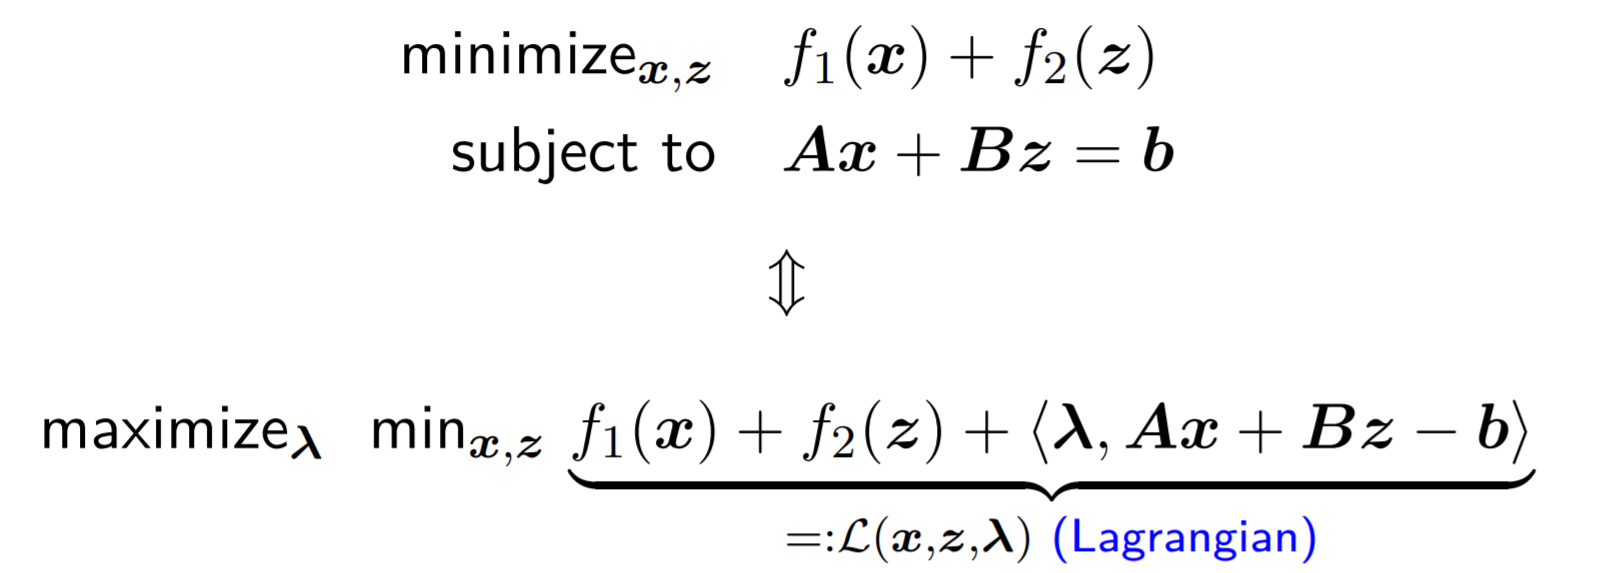
\includegraphics[width=.7\linewidth]{./figs/dual.png}  
	\caption*{}
	%\label{fig:lr_sched}
\end{figure}
	\item The alternating direction method of multipliers (ADMM) solves the above problem by alternating minimizations for $x$ and $z$ and updating the dual variable $\lambda$, i.e., 
	\begin{figure}[H]
		\centering
		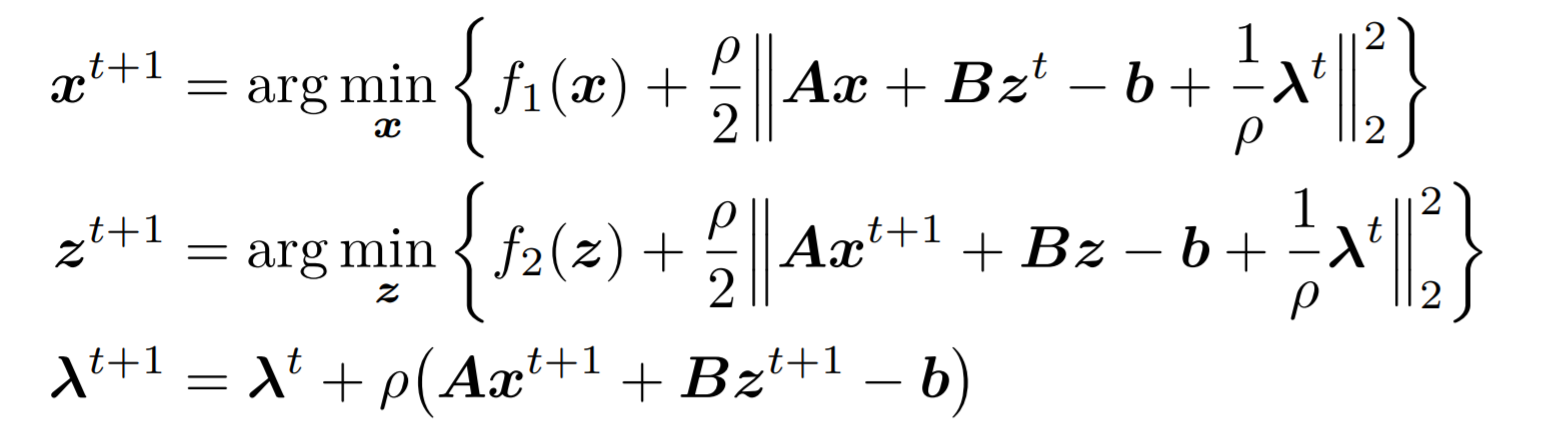
\includegraphics[width=.7\linewidth]{./figs/admm.png}  
		\caption*{}
		%\label{fig:lr_sched}
	\end{figure}	 
	\item Final algorithm
		\begin{figure}[H]
		\centering
		\includegraphics[width=.95\linewidth]{./figs/updates.png}  
		\caption*{}
		%\label{fig:lr_sched}
	\end{figure}
	
\end{itemize}
\section{Experiments}
\begin{enumerate}
	\item Comparison between parallel and cascade frameworks
		\begin{itemize}
	\item FFN $784 \times 300 \times 1000 \times 100 \times 10$ for MNIST
	\item In practice original training data can be used for the retraining phase
	\item Working with less amount of data is computationally desirable
		\begin{figure}[H]
		\centering
		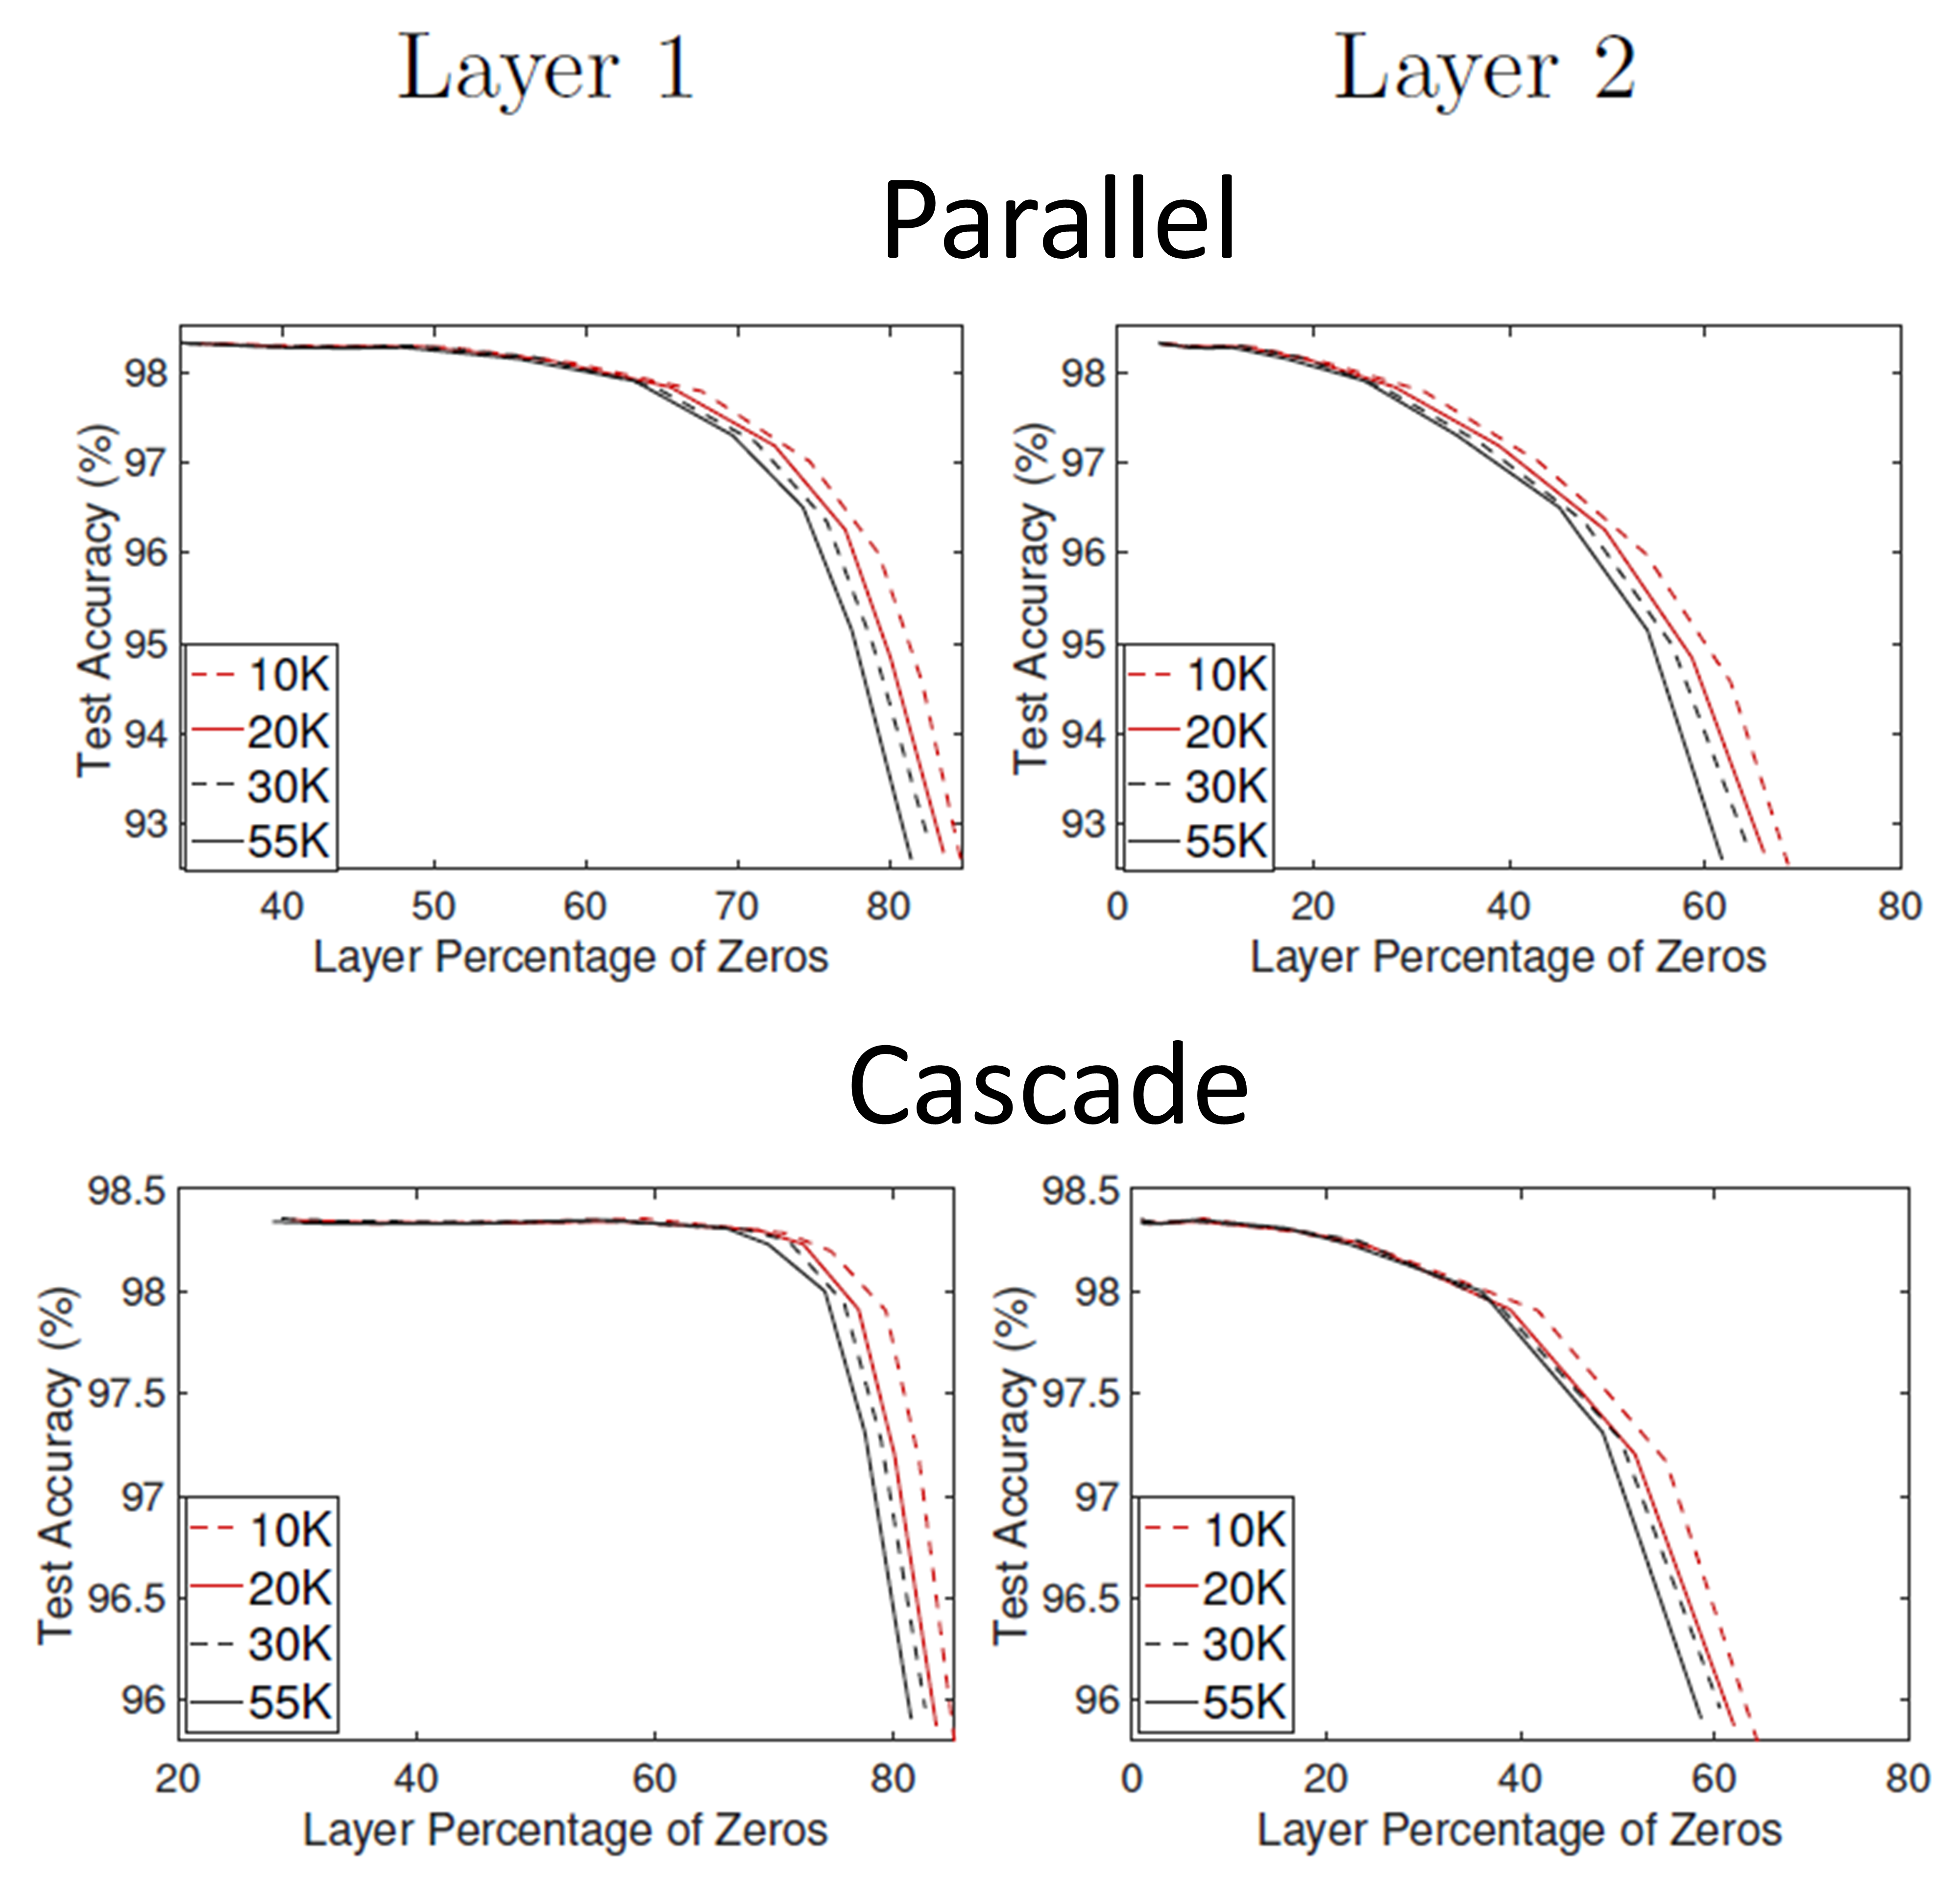
\includegraphics[width=.9\linewidth]{./figs/parallel_vs_cascade.png}  
		\caption*{}
		%\label{fig:lr_sched}
	\end{figure}

		\item Test accuracy drops faster for increasing sparsity for parallel framework
		\item Recall that sparsity is controlled through the allowed discrepancy $\epsilon$
		\item However, parallel is distributable and thus can be faster
	\end{itemize}
\newpage
	\item Comparison of Net-Trim with Dropout and $\ell_1$ penalty
	\begin{itemize}
		\item LeNet convolutional network
			\begin{figure}[H]
			\centering
			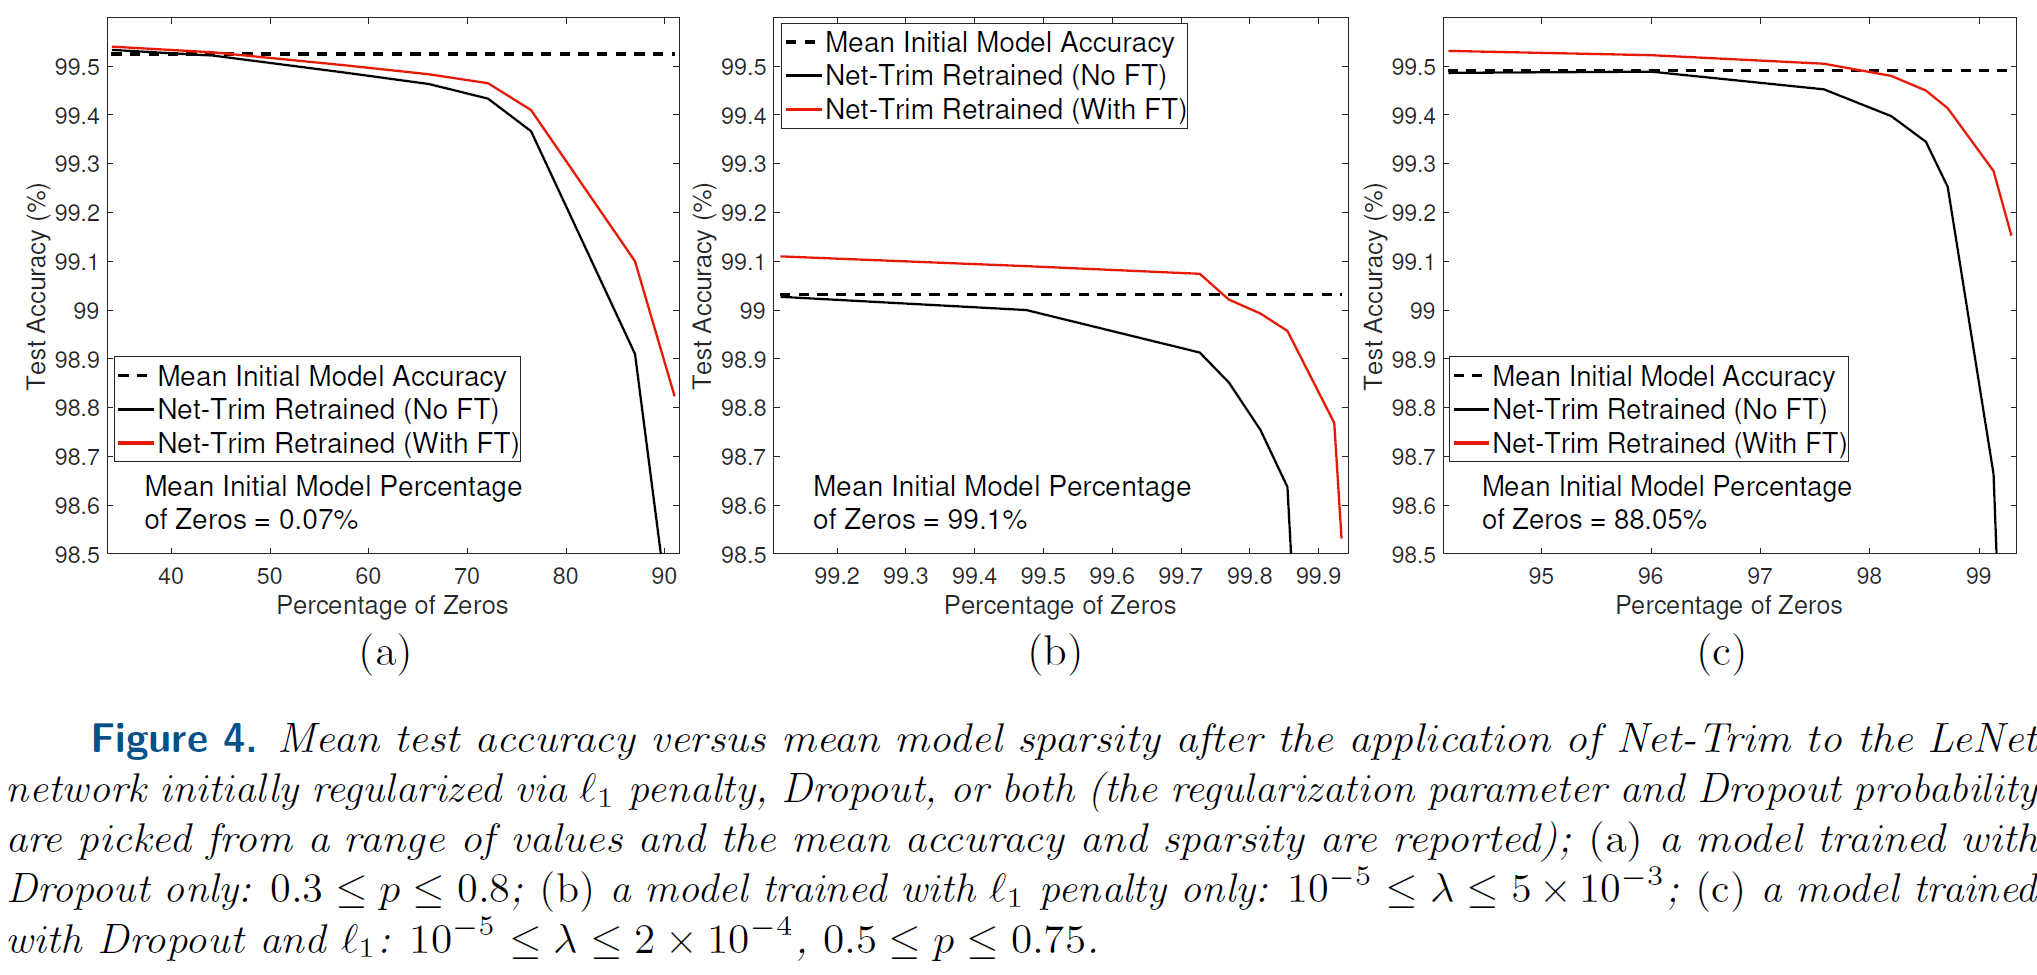
\includegraphics[width=1\linewidth]{./figs/dropout_comp.png}  
			\caption*{}
			%\label{fig:lr_sched}
		\end{figure}
		\item For an initially trained model with Dropout + $l_1$ penalty we can reduce percentage of zeros from $88 \%$ to $98 \%$ without loss of accuracy (panel c)
		\item It seems that with fine-tuning we can even increase accuracy while also pruning the network
	\end{itemize}
\newpage
\item Comparison of Net-Trim with HPTD (\cite{han2015learning}) which truncates the small weights across a trained network and performs another round of training on the active weights (fine-tuning)
\begin{itemize}
	\item FC (top) and LeNet (bottom) networks
	\begin{figure}[H]
		\centering
		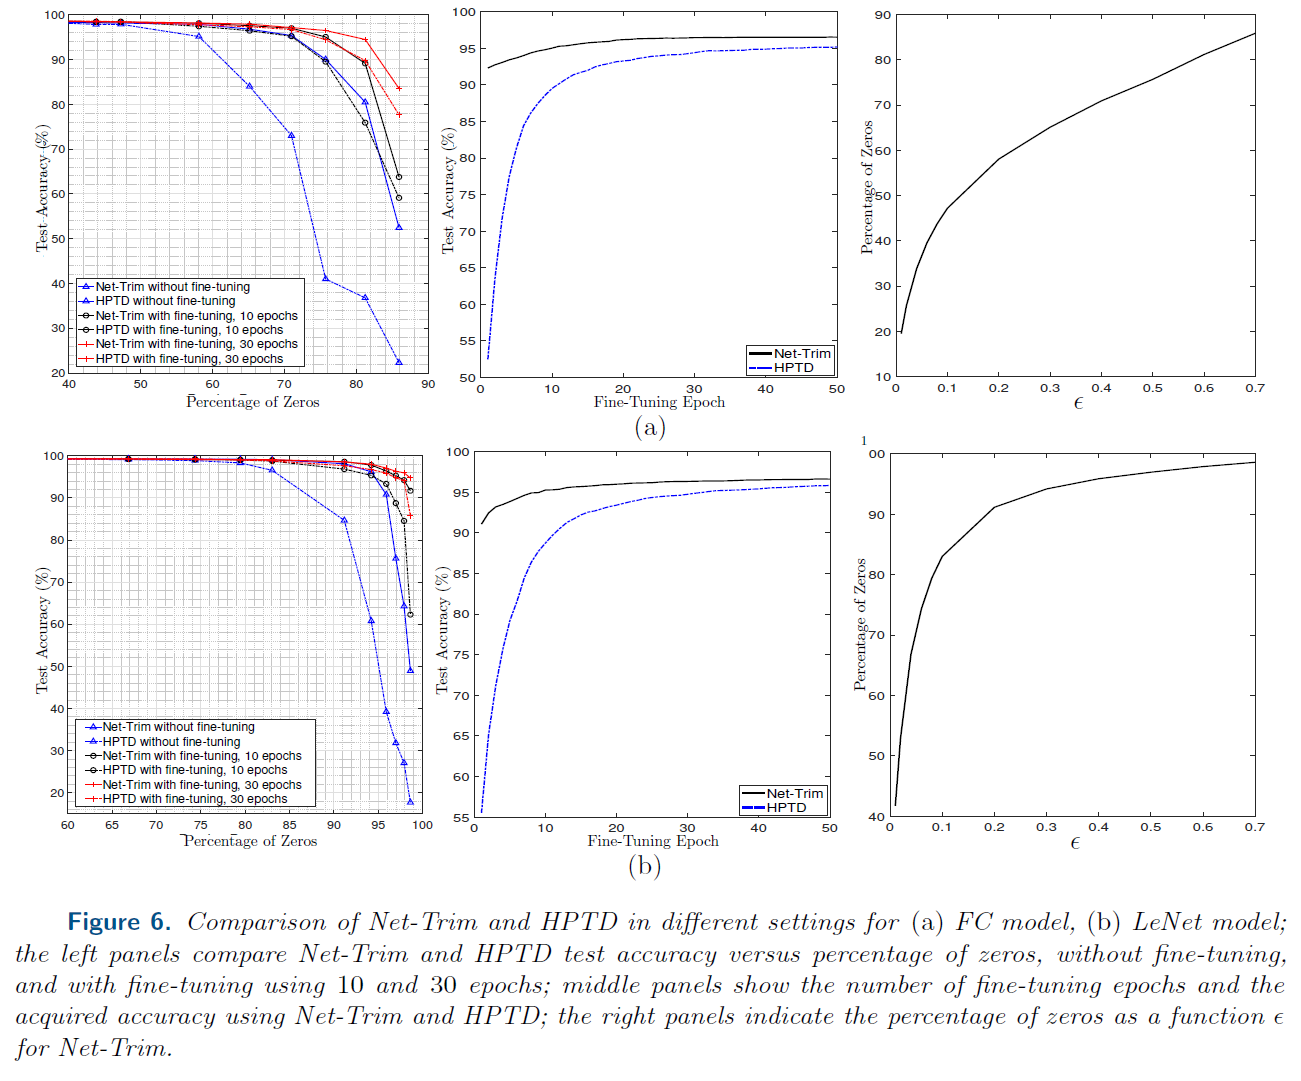
\includegraphics[width=1\linewidth]{./figs/hptd_comp.png}  
		\caption*{}
		%\label{fig:lr_sched}
	\end{figure}
	\item For the Net-Trim we use different values of $\epsilon$  to prune the trained networks. To compare the method with the HPTD, after each application of the Net-Trim and counting the number of zeros, the same number of elements are truncated from the initial network to be used for the HPTD implementation. HPTD is followed by a fine-tuning step after the truncation, which is also an optional task for Net-Trim
	\item Net-Trim outperforms HPTD in these scenarios. The reason is that pruning with HPTD is based on the magnitude of the weights, which in many cases may discard connections to the important features and variables in the network
	\item Applying the Net-Trim to each layer of the MNIST networks is on the order of 20 seconds, and the fine-tuning step is on the order of 30 seconds. For the CIFAR-10 network, the Net-Trim application to each layer is about 1 minute, and the fine-tuning step takes about 20--30 minutes, depending on the sparsity of the network
	\item Discarding weights via HPTD does not incur any computational cost while fine-tuning may take more time compared to Net-Trim (see middle panels in figure above)
	\item Note that fine-tuning may degrade the accuracy especially in low pruning regimes (small percentage of zeros) due to overfitting
\end{itemize}
	
\end{enumerate}






	


%%%%%%%%%%%%%%%%%%%%%%%%%%%%%%%%%%%%%%%%%%%%%%%%%%%%%%%%%%%%%%%%%%%%%%%%%%%%%%%%%%%%%%%%%%%%%%%%%%%%%%%%%	

%\section*{Appendix}
\newpage	
\printbibliography[heading=bibintoc,title={References}]
	
\end{document}